\documentclass{article}

\usepackage{graphicx} % Required for inserting images
\usepackage{amsmath} % useful
\usepackage{amsfonts} % fonts like \mathbb{R} among others
\usepackage{amssymb}
\usepackage{amsthm} % used for writing lemmas/theorems/etc
\usepackage{tikz} % for visual tools
\usepackage{authblk}
\usepackage{enumitem}
\usepackage{url}
\usepackage{subfig}
\usepackage{float} % i hate images
\numberwithin{equation}{section}
\usepackage[margin=1in]{geometry}

\newtheorem{theorem}{Theorem}[section]
\newtheorem{corollary}{Corollary}[theorem]
\newtheorem{lemma}[theorem]{Lemma}
\newtheorem{proposition}[theorem]{Proposition}

\theoremstyle{definition}
\newtheorem{definition}{Definition}[section]
\newtheorem{remark}{Remark}[theorem]

\title{MATH60025 Computational PDEs Coursework 1}
\author{
CID: 02033585
}
\date{}

\newcommand{\R}{\mathbb{R}}
\newcommand{\C}{\mathbb{C}}
\newcommand{\Q}{\mathbb{Q}}
\newcommand{\pr}{\mathbb{P}}
\newcommand{\E}{\mathbb{E}}
\newcommand{\dm}{\mathrm{d}}

\newcommand{\mc}[1]{\mathcal{#1}}
\newcommand{\pspace}{(\Omega, \mathcal{F}, \mathbb{P})}

\newcommand{\sm}{\setminus}

\newcommand{\ie}{\textit{i}.\textit{e}. }
\newcommand{\eg}{\textit{e}.\textit{g}. }

\newcommand{\dd}[2]{\frac{\mathrm{d} #1}{\mathrm{d} #2}}
\newcommand{\ddn}[3]{\frac{\mathrm{d}^{#3} #1}{\mathrm{d}^{#3} #2}}
\newcommand{\pp}[2]{\frac{\partial #1}{\partial #2}}
\newcommand{\ppn}[3]{\frac{\partial^{#1} #2}{\partial^{#1} #3}}


\newcommand{\eps}{\varepsilon}
\begin{document}

\maketitle

\section{Part A}
\subsection{1}
The steady state solution is $u(x,t) = 0$. This can be found by setting $u_t$ to $0$, since the solution shouldn't change in time. This means that $u_{xx} = 0$, meaning that $u(x,t) = ax + b$ for some constants $a$ and $b$. By applying the boundary conditions, we find that $a = 0$ and $b = 0$, hence the result.

\subsection{2}

First, assume seperability \ie $u(x,t) = X(x)T(t)$. Then, 
\begin{align}
    u_t = X(x)T'(t) \\
    u_{xx} = X''(x)T(t) \\
    \frac{T'(t)}{T(t)} = \frac{X''(x)}{X(x)}
\end{align}
Since the above holds for all $t$ and $x$, both sides must be a constant, which we denote $\lambda$.

We can then use standard techniques to solve the two ODEs given by
\begin{align}
    T'(t) = \lambda T(t) \\
    X''(x) = \lambda X(x)
\end{align}

If $\lambda \geq 0$, then the solution to the PDE is 

\begin{equation}
    u(x,t) = e^{\lambda t} (C_1 \sinh(\sqrt{\lambda} x) + C_2 \cosh(\sqrt{\lambda} x))
\end{equation}
which we see cannot satisfy the boundary conditions for $t>0$ unless $u$ is the zero solution. Hence, we consider $\lambda < 0$ instead. The solution is then

\begin{equation}
    u(x,t) = e^{\lambda t} (C_1 \sin(\sqrt{-\lambda} x) + C_2 \cos(\sqrt{-\lambda} x))
\end{equation}

We now find out suitable values for $\lambda$ that satisfy the boundary conditions. Since $u(0,t) = 0$, we have $C_2 = 0$ and reduce our solution to $Ce^{\lambda t} \sin(\sqrt{-\lambda}x)$, which always satisfies the condition at the boundary $x=0$. For the other boundary $x=1$, we need $\sin(\sqrt{-\lambda}) = 0$, resulting in 
\begin{equation}
    \lambda = -n^2 \pi^2 \text{ for } n \in \mathbb{N}
\end{equation}

and solutions $u_n(x,t) = e^{-n^2 \pi^2 t} \sin(n\pi x)$.

We will satisfy the initial condition by expanding in a fourier series and superimposing our solutions (as the PDE is linear).

We expand $f(x)=1$ in terms of a fourier series, whose coefficients $a_n$ can be computed using the inner product

\begin{equation}
    a_n = \frac{\int_{0}^{1}f\left(x\right)\sin\left(\pi nx\right)dx}{\int_{0}^{1}\sin\left(\pi nx\right)^{2}dx} = \left\{\begin{matrix}
        \frac 4{\pi n} & \text{if $n$ is odd}\\ 
        0 & \text{otherwise}
        \end{matrix}\right.
\end{equation}

We then sum the solutions corresponding to the fourier modes together to get the solution satisfying all the right boundary/initial conditions:

\begin{equation}
    u(x,t) = \sum_{k=0}^{\infty} a_k u_k(x,t) = \frac {4}{\pi} \sum_{n=0}^{\infty} \frac{1}{2n+1} e^{-(2n+1)^2 \pi^2 t} \sin((2n+1)\pi x)
\end{equation}

\subsection{3}
We use the finite difference approximations on a mesh with $N$ points in the $x$ direction, with $u_n^j$ denoting the $n$th point in the direction of $x$ and the $j$th point in the $t$ direction. We then have

\begin{align}
    \frac{u_n^{j+1} - u_n^j}{k} = \pp{u_n^j}{t} + O(k) \\
    \frac{u_{n+1}^j - 2u_n^j + u_{n-1}^j}{h^2} = \ppn{2}{u_n^j}{x} + O(h^2)
\end{align}
By equating the two derivatives per the PDE, we get the numerical scheme, which has a truncation error that is $O(k)$ and $O(h^2)$.

\begin{equation}
    U_n^{j+1} = rU_{n+1}^j + (1-2r)U_n^j + rU_{n-1}^j
\end{equation}
where $r = \frac{k}{h^2}$.

We set all $U_0^j$ and $U_N^j$ to $0$ for $j>0$ and all $U_1^0, \dots, U_{N-1}^0$ to $1$ to encode the boundary conditions.

Relevant code: \path{q3A}

\begin{figure}[H]\
    \centering
    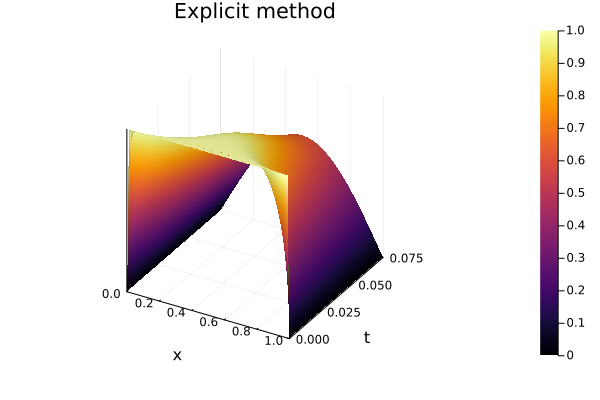
\includegraphics[width=0.46\textwidth]{qA3.png}
    \caption{Contour of the solution with the Explicit method on a $101 \times 2001$ grid.}
    \label{fig:afig_e}
\end{figure}

\subsection{4}

\begin{figure}[H]
    \centering
    \subfloat[Error with $h$ fixed and $k$ varying]{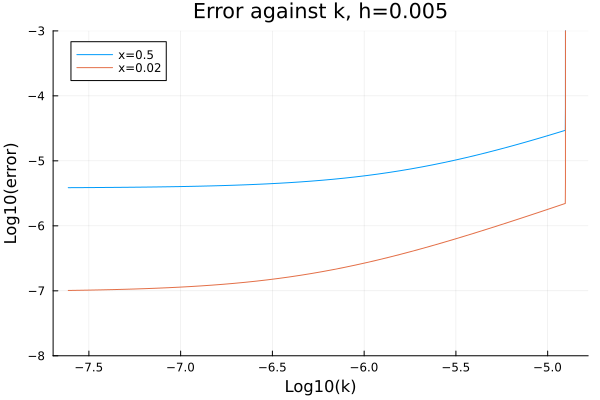
\includegraphics[width=0.46\textwidth]{qA4_1.png}}\hfill
    \subfloat[Error with $h$ fixed and $r$ varying]{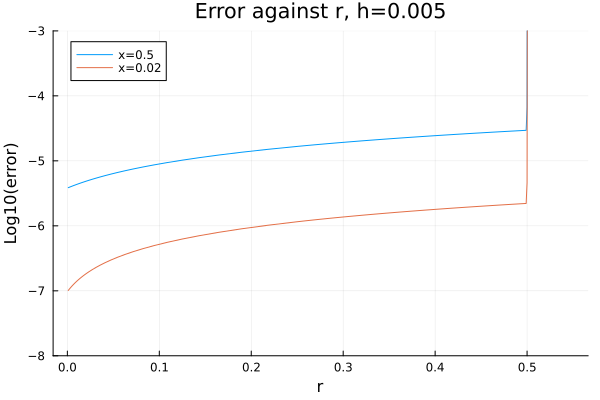
\includegraphics[width=0.46\textwidth]{qA4_2.png}} \\
    \subfloat[Error with $k$ fixed and $h$ varying]{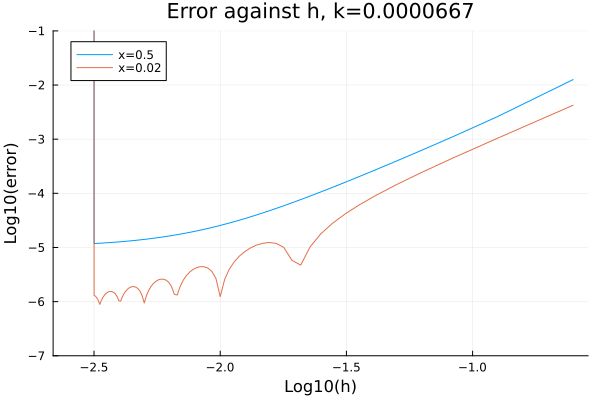
\includegraphics[width=0.46\textwidth]{qA4_3.png}}\hfill
    \subfloat[Error with $k$ fixed and $r$ varying]{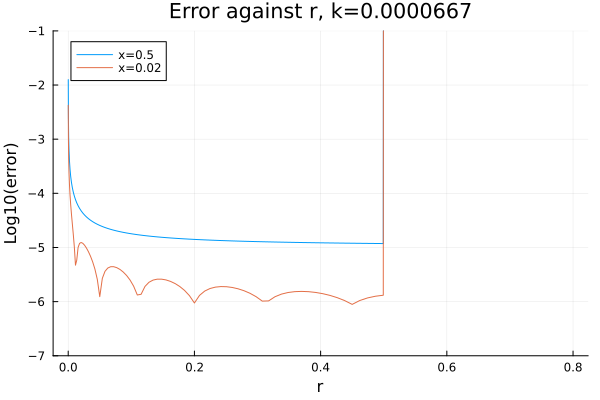
\includegraphics[width=0.46\textwidth]{qA4_4.png}}
    \caption{Investigation of error with varying $h$, $k$ and $r$, at points $x=0.5$ (Blue) and $x=0.02$ (Orange).}
    \label{fig:afig1}
\end{figure}
In Figure \ref{fig:afig1}, we investigate the error of the computed solution and the analytic solution at the points $x=0.5$ and $x=0.02$ with $t=0.075$. In (b) and (d), we see the critical value of $r=0.5$ where the scheme transitions from stable to unstable.

We see in (a) and (b) that as $k \to 0$, the error is decreasing. In (a), the gradient of the lines near $\log_{10}(k) \approx -5.0$ right hand side is close to $1$, reflecting that the truncation error in the scheme is $O(k)$. The leveling off near $\log_{10}(k) \approx -7.5$ is due to the fact that the truncation error is actually $O(k + h^2)$ and the $O(h^2)$ component begins to dominate the truncation error.

Similarly, with (c) we can see that the gradient of the lines is close to $2$, reflecting the $O(h^2)$ behaviour of the truncation error. In (d) we see a tradeoff in the value of $h$. If $h$ is too big, we lose accuracy due to large truncation error, despite the scheme being stable. On the other hand, if $h$ is too small, $r$ becomes bigger than $0.5$ and we lose stability.

The error is less at $x=0.02$ than $x=0.5$ due to the dependence of the truncation error on $x$ and $t$. More specifically, the truncation error here is
\begin{equation}
    R_n^j = \frac 1{12} h^2 \ppn{4}{u_n^j}{x} - \frac 12 k \ppn{2}{u_n^j}{t} + O(k^2, h^4)
\end{equation}
Note that under the assumption of smoothness of the solution, $u_{xxxx} = u_{tt}$. Hence the error is linear in the value of $u_{tt}$ at the point.

We can calculate $u_{tt}$ using the analytic solution, revealing that $u_{tt}(0.02, 0.075) \approx 4.517$ whilst $u_{tt}(0.5, 0.075) \approx 54.881$. This explains why the error is an order of magnitude higher for $x=0.5$ than $x=0.02$.

The weird patterns in the $x=0.02$ case occur because the number of spacing points $N$ doesn't align with the $x$ value, and instead the calculated value is done via linear interpolation.

\subsection{5}
We consider measuring log-relative accuracy with respect to $u_{tt}$, defined as
\begin{equation}
    error = \log_{10}\left| \frac{u_{numerical} - u_{analytic}}{u_{tt,analytic}} \right|
\end{equation}

\begin{figure}[H]
    \centering
    \subfloat[Error with $h$ fixed and $k$ varying]{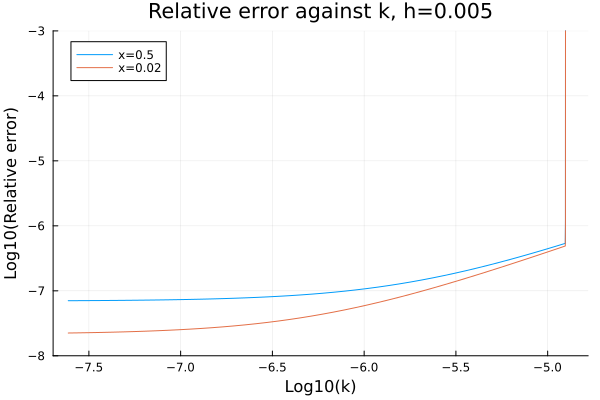
\includegraphics[width=0.46\textwidth]{qA5_1.png}}\hfill
    \subfloat[Error with $h$ fixed and $r$ varying]{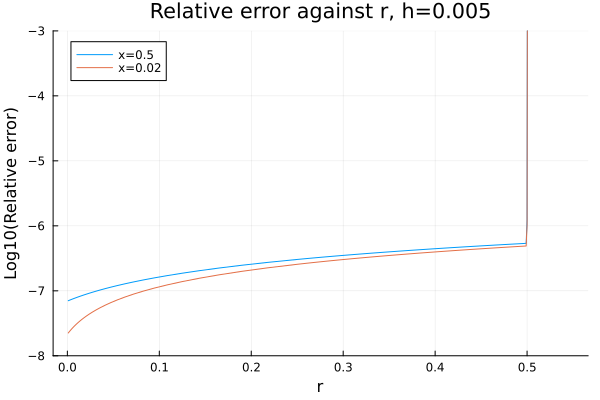
\includegraphics[width=0.46\textwidth]{qA5_2.png}} \\
    \subfloat[Error with $k$ fixed and $h$ varying]{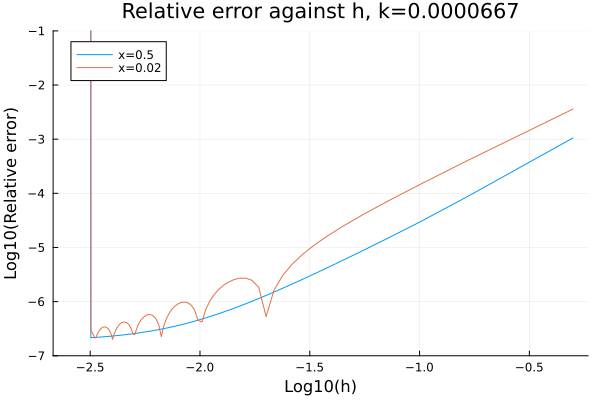
\includegraphics[width=0.46\textwidth]{qA5_3.png}}\hfill
    \subfloat[Error with $k$ fixed and $r$ varying]{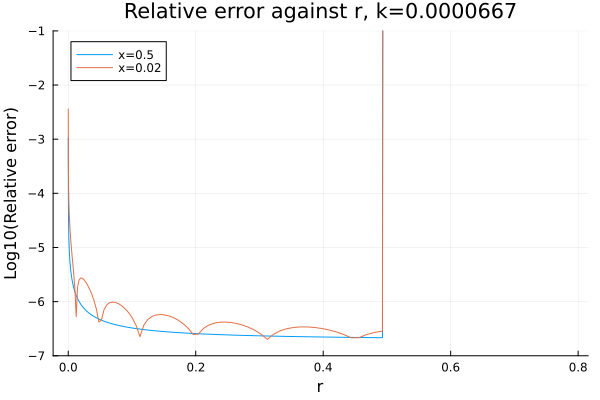
\includegraphics[width=0.46\textwidth]{qA5_4.png}}
    \caption{Investigation of relative error with varying $h$, $k$ and $r$, at points $x=0.5$ (Blue) and $x=0.02$ (Orange).}
    \label{fig:afig2}
\end{figure}

We see that after rescaling by the partial derivative $u_{tt}$ (which was calculated via the analytic solution), the lines are much closer to each other now and the error for both $x=0.02$ and $x=0.5$ behave similarly now, whilst maintaining the features described in the previous question.

\subsection{6}
The scheme we will be using is described as follows
\begin{equation}
    U_n^{j+1}-U_n^j = \frac r2 (\delta^2 U_n^{j+1} + \delta^2 U_n^j)
\end{equation}
which we rearrange into a linear system with tridiagonal matrices as follows
\begin{equation}
    U_n^{j+1}-U_n^j = \frac r2 \left(U_{n+1}^{j+1} -2U_{n}^{j+1} + U_{n-1}^{j+1} + U_{n+1}^{j} -2U_{n}^{j} + U_{n-1}^{j}\right)
\end{equation}
\begin{equation}
    \left(1+r\right)U_{n}^{j+1}-\frac{r}{2}U_{n+1}^{j+1}-\frac{r}{2}U_{n-1}^{j+1}=\left(1-r\right)U_{n}^{j}+\frac{r}{2}U_{n+1}^{j}+\frac{r}{2}U_{n-1}^{j}
\end{equation}
resulting in the following system. Here, we are using $U^j = [U_1^j, \dots, U_{N-1}^j]$
\begin{equation}
    AU^{j+1} = BU^j 
\end{equation}
where

\begin{equation}
    A = \begin{bmatrix}
        1+r & -\frac r2 &  & \\ 
        -\frac r2 & 1+r & \ddots & \\ 
         & \ddots & \ddots & -\frac r2\\ 
         &  & -\frac r2 & 1+r
        \end{bmatrix}
        \hspace{1cm}
        B = \begin{bmatrix}
        1-r & \frac r2 &  & \\ 
        \frac r2 & 1-r & \ddots & \\ 
         & \ddots & \ddots & \frac r2\\ 
         &  & \frac r2 & 1-r
        \end{bmatrix}
\end{equation}
Relevant code: \path{qA6}

\begin{figure}[H]\
    \centering
    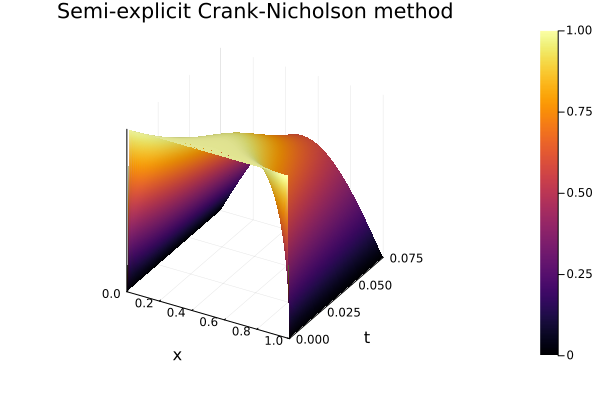
\includegraphics[width=0.46\textwidth]{qA6.png}
    \caption{Contour of the solution with the Semi-explicit Crank-Nicholson method on a $101 \times 2001$ grid.}
    \label{fig:afig_se}
\end{figure}


\subsection{7}


\begin{figure}[H]
    \centering
    \subfloat[Error with $h$ fixed and $k$ varying]{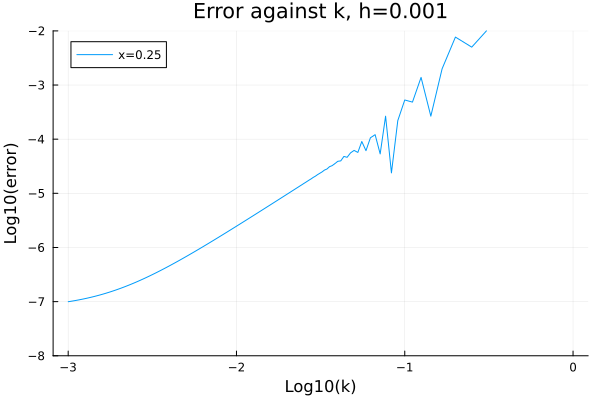
\includegraphics[width=0.46\textwidth]{qA7_1.png}}\hfill
    \subfloat[Error with $h$ fixed and $r$ varying]{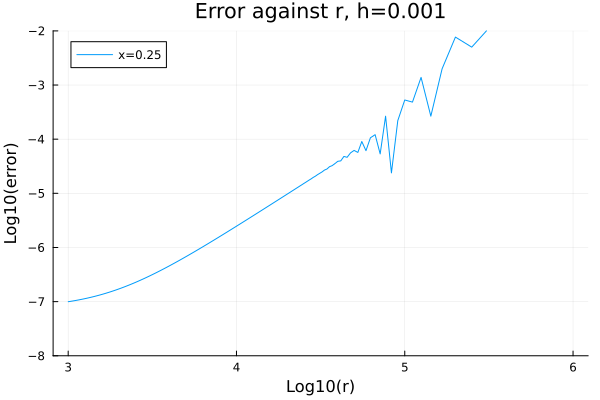
\includegraphics[width=0.46\textwidth]{qA7_2.png}} \\
    \subfloat[Error with $k$ fixed and $h$ varying]{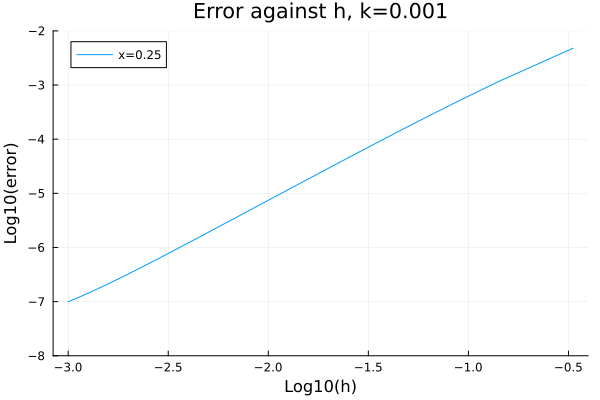
\includegraphics[width=0.46\textwidth]{qA7_3.png}}\hfill
    \subfloat[Error with $k$ fixed and $r$ varying]{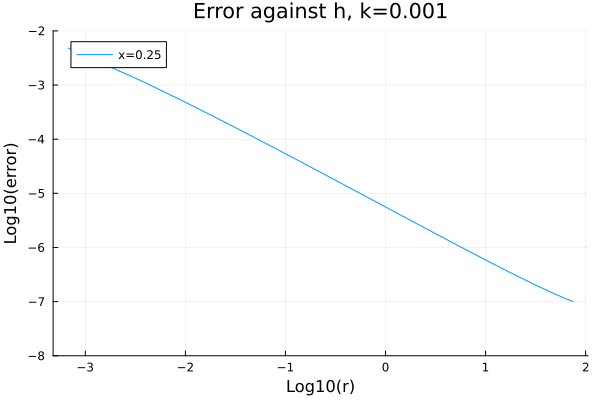
\includegraphics[width=0.46\textwidth]{qA7_4.png}}
    \caption{Investigation of relative error with varying $h$, $k$ and $r$, at point $x=0.25$ (Blue).}
    \label{fig:afig3}
\end{figure}

The figures in Figure \ref{fig:afig3} above were done similarly to before, fixing $h,k,r$ whilst varying another parameter. The main differences to note here are
\begin{itemize}
    \item The gradient of all lines present is $2$, which reflects the truncation error being of order $O(h^2,k^2)$ rather than $O(h^2, k)$ previously. The change can be seen in (a)
    \item Since the scheme is unconditionally stable, the scheme can have very large values of $r$ and still be stable (b) (d). There is no transition point anymore.
    \item In general, we do not need $k$ to be so small anymore to achieve sufficient accuracy. Here, $k = 10^{-3}$ was used in (c) and (d) to achieve $7$ digits, whilst previously we needed $k < 10^{-6}$. This is a consequence of the improved truncation error from $O(k)$ to $O(k^2)$.
\end{itemize}

Hence, the better technique is the semi-explicit method Crank-Nicholson method, as we can achieve similar accuracy with higher values of $k$ in particular. In addition, we no longer need to worry about stability and can choose a much smaller grid size. This greatly outweighs the cost to solve a tridiagonal system many times in terms of computational time.

\section{B}
\subsection{1}
The solution to the PDE is approximated by $U_n^j$ on the grid $(x_n, t^j)$ with spacings $h$ and $k$ respectively. To find the order of the truncation error, we first recall the results derived from Taylor series of partial derivatives.
\begin{align}
    \label{eq:btaylor}
    \frac{u_n^{j+1} - u_n^{j-1}}{2k} = \pp{u_n^j}{t} +\frac 16 k^2 \ppn{3}{u_n^j}{x} + O(k^4)\\
    \frac{u_{n+1}^j - 2u_n^j + u_{n-1}^j}{h^2} = \ppn{2}{u_n^j}{x} + \frac{1}{12} h^2 \ppn{4}{u_n^j}{x} + O(h^4)
\end{align}
By setting the partial derivatives equal according to the PDE, we get
\begin{equation}
    \label{eq:bundiscretised}
    \frac{u_n^{j+1} - u_n^{j-1}}{2k} = \frac{u_{n+1}^j - 2u_n^j + u_{n-1}^j}{h^2}  +R_n^j
\end{equation}
where the truncation error $R_n^j$ is
\begin{equation}
    \label{eq:btrunc}
    R_n^j = \frac{1}{12} h^2 \ppn{4}{u_n^j}{x} + O(h^4) - \frac 16 k^2 \ppn{3}{u_n^j}{x} + O(k^4)
\end{equation}
Thus, the order of the trunctation error is $O(h^2, k^2)$. We now use the Fourier method to investigate the stability. Denote the error to be $z_n^j = u_n^j - U_n^j$.

Suppose that at $t=0$, there is a small error in the numerical and analytic solution $z_n^0 = \eps e^{inph}$, where $p$ is a spatial wavenumber. We only consider the effect of a small complex exponential perturbation, since we can reconstruct any other initial data pertubation using fourier series.

Then after using Equation \eqref{eq:bundiscretised} and the numerical scheme (by subtracting one from another), the error $z_n^j$ satisfies the equation
\begin{equation}
    \frac{z_n^{j+1} - z_n^{j-1}}{2k} = \frac{z_{n+1}^j - 2z_n^j + z_{n-1}^j}{h^2} + R_n^j
\end{equation}
resulting in the equation for $z_n^{j+1}$, where we neglected the trunctation error term and used $r = \frac{k}{h^2}$
\begin{equation}
    z_n^{j+1} = z_n^{j-1} + 2r(z_{n+1}^j - 2z_n^j + z_{n-1}^j)
\end{equation}
Now suppose that the solution to the recursive formula above is seperable \ie $z_n^j = \eps \xi_j e^{inph}$ for some sequence $\xi_j$ with $\xi_0 = 1$. Hence we derive a recursion relation below.

\begin{equation}
    \eps \xi_{j+1} e^{inph} = \eps \xi_{j-1} e^{inph} + 2r(\eps \xi_j e^{i(n+1)ph} - 2\eps \xi_j e^{inph} + \eps \xi_j e^{i(n-1)ph})
\end{equation}
\begin{equation}
     \xi_{j+1}  =  \xi_{j-1}  + 2r( \xi_j e^{iph} - 2 \xi_j  + \xi_j e^{-iph})
\end{equation}
\begin{equation}
    \xi_{j+1}  =  \xi_{j-1} + 4r (\cos(ph) - 1) \xi_j
\end{equation}
\begin{equation}
    \xi_{j+1}  =  \xi_{j-1} -8r\sin^2\left(\frac{ph}{2}\right) \xi_j
\end{equation}
To solve this difference equation, we try the ansatz $ \xi_j = \lambda^j$. Upon substitution, we have
\begin{equation}
    \lambda^{j+1}=\lambda^{j-1}-8r\sin^{2}\left(\frac{ph}{2}\right)\lambda^{j}
\end{equation}
from which the characteristic equation has solutions
\begin{align}
    \lambda_1 = -4r\sin^{2}\left(\frac{ph}{2}\right) + \sqrt{16r^{2}\sin^{4}\left(\frac{ph}{2}\right)+1} \\
    \lambda_2 = -4r\sin^{2}\left(\frac{ph}{2}\right) - \sqrt{16r^{2}\sin^{4}\left(\frac{ph}{2}\right)+1}
\end{align}
and general solution $A \lambda_1^j + B \lambda_2^j$. In order for the errors to not grow, we need both $|\lambda_1| \leq 1$ and $|\lambda_2| \leq 1$.
If $ph = \pi$, we have

\begin{equation}
    |\lambda_2| = 4r+\sqrt{16r^{2}+1} > 1
\end{equation}
Hence, for any value of $r>0$, the errors grow and the scheme is not stable.

\subsection{2}
We need the following finite difference formulas derived from Taylor series
\begin{align}
    \label{eq:btaylor2}
    \frac{u_n^{j+1} - u_n^{j-1}}{2k} = \pp{u_n^j}{t} +\frac 16 k^2 \ppn{3}{u_n^j}{x} + O(k^4)\\
    \frac{u_{n+1}^j - 2u_n^j + u_{n-1}^j}{h^2} = \ppn{2}{u_n^j}{x} + \frac{1}{12} h^2 \ppn{4}{u_n^j}{x} + O(h^4) \\
    \frac{u_{n}^{j+1} - 2u_n^j + u_{n}^{j-1}}{k^2} = \ppn{2}{u_n^j}{t} + \frac{1}{12} k^2 \ppn{4}{u_n^j}{t} + O(k^4)
\end{align}
By multiplying the third formula by $\frac{k^2}{h^2}$ and subtracting it from the second, we have
\begin{equation}
    \frac{u_{n+1}^j - u_{n}^{j+1} - u_{n}^{j-1} + u_{n-1}^j}{h^2} = \ppn{2}{u_n^j}{x} + \frac{1}{12} h^2 \ppn{4}{u_n^j}{x} + O(h^4) - \frac{k^2}{h^2}\left(\ppn{2}{u_n^j}{t} - \frac{1}{12} k^2 \ppn{4}{u_n^j}{t} + O(k^4)\right)
\end{equation}
Equating partial derivatives according to the PDE yields
\begin{equation}
    \frac{u_{n+1}^j - u_{n}^{j+1} - u_{n}^{j-1} + u_{n-1}^j}{h^2} = \frac{u_n^{j+1} - u_n^{j-1}}{2k} + R_n^j
\end{equation}
where we denote the truncation error as $R_n^j$, which is equal to
\begin{equation}
    R_n^j = - \frac 16 k^2 \ppn{3}{u_n^j}{x} + \frac{1}{12} h^2 \ppn{4}{u_n^j}{x} + O(k^4, h^4) - \frac{k^2}{h^2}\left(\ppn{2}{u_n^j}{t} - \frac{1}{12} k^2 \ppn{4}{u_n^j}{t} + O(k^4)\right)
\end{equation}
From this we see that in order for $R_n^j$ to go to $0$ as $h \to 0$ and $k \to 0$, we also need $ \frac kh$ to go to $0$, or equivalently $k = o(h)$.

\subsection{3}
The basis we will use in the application of the Fourier method is $e^{ilp_x h_x}e^{imp_y h_y}e^{inp_z h_z}$ where $p_x, p_y, p_z$ are wavenumbers in each of the respective directions. As such, we will assume a small exponential perturbation at time $t=0$ with $z_{lmn}^0 = \eps e^{ilp_x h_x}e^{imp_y h_y}e^{inp_z h_z}$, and assume seperability of the solution \ie $z_{lmn}^j = \xi_j z_{lmn}^0$ for some sequence $\xi_j$ with $\xi_0 = 1$.

First, we will calculate the action of the second order central difference operator on a single term.

\begin{align}
    \delta_x^2 z_{lmn}^{j} &= z_{l+1 mn}^{j} - 2z_{lmn}^{j} + z_{l-1 mn}^{j} \\
    &= \eps \xi_j e^{ilp_x h_x}e^{imp_y h_y}e^{inp_z h_z} (e^{ip_x h_x} - 2 + e^{-ip_x h_x}) \\
    &= \xi_j z_{lmn}^0 (2\cos(p_x h_x)-2)
\end{align}
A similar calculation can be done for $\delta_y^2, \delta_z^2$ and also with $z_{lmn}^{j+1}$ with just an exchange of indices.

Thus, since the errors also follow the same recursion relation as the scheme up to ignoring truncation errors, we have

\begin{equation}
    z_{lmn}^{j+1} - z_{lmn}^j = k \left[
        \frac{1}{h_x^2}\delta_x^2 + 
        \frac{1}{h_y^2}\delta_y^2 + 
        \frac{1}{h_z^2}\delta_z^2
    \right]
    \left(
        \theta z_{lmn}^{j+1} + (1-\theta)z_{lmn}^j
    \right)
\end{equation}

\begin{equation}
    \xi_{j+1}z_{lmn}^0 - \xi_j z_{lmn}^0 = k z_{lmn}^0
        \left(\theta \xi_{j+1} + (1- \theta) \xi_j\right) \left(
            \frac{2\cos(p_x h_x)-2}{h_x^2} +
            \frac{2\cos(p_y h_y)-2}{h_y^2} +
            \frac{2\cos(p_z h_z)-2}{h_z^2}
        \right)
\end{equation}
    
\begin{equation}
    \xi_{j+1} - \xi_j  = k
        \left(\theta \xi_{j+1} + (1- \theta) \xi_j\right)A_{xyz}
\end{equation}
where we defined

\begin{equation}
    A_{xyz} = A(p_x, h_x, p_y, h_y, p_z, h_z) = \left(
    \frac{2\cos(p_x h_x)-2}{h_x^2} +
    \frac{2\cos(p_y h_y)-2}{h_y^2} +
    \frac{2\cos(p_z h_z)-2}{h_z^2}
\right)
\end{equation}
We substitute the ansatz $\xi_j = \lambda^j$ to the linear difference equation.
\begin{equation}
    \lambda^{j+1} - \lambda^j  = k
        \left(\theta \lambda^{j+1} + (1- \theta) \lambda^j\right)A_{xyz}
\end{equation}
\begin{equation}
    \lambda - 1  = k
        \left(\theta \lambda + (1- \theta) \right)A_{xyz}
\end{equation}
\begin{equation}
    \lambda = \frac{1 + k(1- \theta)A_{xyz}}{1 - k \theta  A_{xyz}} = 1 + \frac{kA_{xyz}}{1 - k \theta  A_{xyz}}
\end{equation}

We require $|\lambda| \leq 1$ for stability. This is equivalent to the condition that 
\begin{equation}
    \label{eq:bequivcondition}
    -2 \leq \frac{kA_{xyz}}{1 - k \theta  A_{xyz}} \leq 0
\end{equation}
Note that we have the following bounds on $A_{xyz}$:
\begin{equation}
    -4 \left( \frac{1}{h_x^2} +
    \frac{1}{h_y^2} +
    \frac{1}{h_z^2}\right) \leq A_{xyz} \leq 0
\end{equation}

Therefore, continuing on from \eqref{eq:bequivcondition}, since $1 - k \theta  A_{xyz}$ is always positive and non-zero, we have
\begin{equation}
    -2(1 - k \theta  A_{xyz})\leq kA_{xyz} \leq 0
\end{equation}
The second inequality always holds, so we drop it here.
\begin{equation}
    -2 + 2 k \theta  A_{xyz}\leq kA_{xyz}
\end{equation}
\begin{equation}
    -2 \leq kA_{xyz} (1- 2\theta)
\end{equation}
If $\theta \in [\frac 12, 1]$, then the RHS is always positive (since $A_{xyz} \leq 0$) and the inequality always holds. Hence for these values of $\theta$, the scheme is unconditionally stable.
If $\theta \in [0, \frac 12)$, then for stability, we need
\begin{equation}
    \frac{2}{1- 2\theta} \geq -kA_{xyz} 
\end{equation}
Since the inequality must hold for all values of $A_{xyz}$, in particular for the worst case $A_{xyz} = -4 \left( \frac{1}{h_x^2} +
\frac{1}{h_y^2} +
\frac{1}{h_z^2}\right)$ when $p_x h_x = p_y h_y = p_z h_z = \pi$, we have

\begin{equation}
    \frac{2}{1- 2\theta} \geq 4k \left( \frac{1}{h_x^2} +
    \frac{1}{h_y^2} +
    \frac{1}{h_z^2}\right)
\end{equation}

which can be rearranged into the result

\begin{equation}
    k \left( \frac{1}{h_x^2} +
    \frac{1}{h_y^2} +
    \frac{1}{h_z^2}\right) \leq \frac{1}{2(1- 2\theta)}
\end{equation}


\end{document}